\ylDisplay{Elektriskeem} % Ülesande nimi
{Tundmatu autor} % Autor
{lahtine} % Voor
{2006} % Aasta
{G 2} % Ülesande nr.
{4} % Raskustase
{
% Teema: Elektriahelad
\ifStatement
Leida laengud $q_1$, $q_2$ ja $q_3$ kõikidel skeemil toodud kondensaatoritel.

\begin{center}
	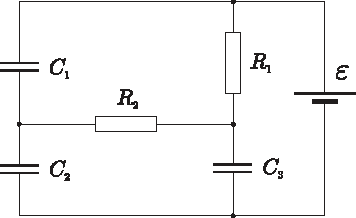
\includegraphics[width=0.7\linewidth]{2006-lahg-02-yl}
\end{center}
\fi


\ifHint
Kuna süsteemi stabiilses olekus on kondensaatorite pinge konstantne ei läbi neid ka vool.
\fi


\ifSolution
Kondensaatori $C_1$ plaadid on ühendatud läbi takistite $R_1$ ja $R_2$. Seepärast laeng selle kondensaatori plaatidel on $q_1 = 0$ (pärast seda, kui on lõppenud kondensaatorite $C_2$ ja $C_3$ laadimine). Kuna pärast kondensaatorite laadimist voolud skeemis ei kulge, pinged kondensaatoritel $C_2$ ja $C_3$ on võrdsed $\mathcal E$. Järelikult, $q_2 = C_2\mathcal E$ ja $q_3 = C_3\mathcal E$. 
\fi
}